% \section{Overview of AI}
% 
% Artificial Intelligence (AI) has been one of the main research subjects over the years due to its 
% potential capabilities to provide solutions to many real-world problems. Its applications include 
% autonomous vehicles, voice assistants, fraud detection, personalized recommendations and so on. 
% Since the application space is vast and there are many researchers working on the field, it is not 
% a surprise to see such big advancements in this field. However, advancements on AI has not been 
% one steep upward climb throughout the history. After Church-Turing thesis, a set of computing 
% machines (computers) were known to be capable of doing any kind of formal reasoning through symbol 
% manipalutions. Such machines are classified as \textit{Universal Turing Machines} or \textit{Turing 
% complete} machines. This realization gave a birth to the bigger vision of creating intelligent 
% machines. To achieve this goal, the community mainly decided to go with one of two approaches 
% starting from 1950: \textbf{symbolic AI} and \textbf{connectionist AI}. 
% 
% Symbolic AI incorporated all the approaches that used high-level representations to solve 
% real-world problems. For many years, symbolic methods were very 
% dominant and was believed to achieve \textit{artificial general intelligence}. Although it was not 
% the case, it has been very useful to develop many symbolic approaches to solve real-world problems. 
% Use of heuristics to optimize within the search space were also closely related to symbolic 
% approaches. At the end of the day, intelligence can also be viewed as an efficient exploration of 
% a search space.
% 
% Connectionist AI approaches used low-level representations in a distributed manner which were to 
% become high-level collectively. Frank Rosenblatt used Perceptron as a simple model of a biological 
% neuron in an attempt to reproduce brain-like behaviour. Although it was very motivating and 
% inspiring attempt, there did not exist enough additional tools (i.e, backpropagation had not been 
% invented yet) to make it work in a scale that artificial neural networks can work nowadays.
% 
% The distinction between these two visions in AI are also viewed as mind-brain dualism. Symbolic AI 
% aims to develop ``mind-like'' approaches whereas connectionist or subsymbolic AI focuses more on 
% the brain side. Many subfields emerged as a reason of an attempt to make machines intelligent. 
% Nowadays, AI has several subfields and some of them are shown below:
% 
% \begin{itemize}
% 	\item \textbf{Evolutionary Computation.} (1950-1960) \newline
% 		Inspired by biological evolution, the main goal of the subfield is a global optimization 
% 		by mimicing process(es) of the evolution. More specifically, the methodologies in 
% 		evolutionary computation requires problem-independent metaheuristics which has inherent 
% 		stochasticity by their nature.
% 	\item \textbf{Expert Systems.} (1970) \newline
% 		Such systems try to emulate human experts by using rule (``if-else'') based algorithms. 
% 		The main components of experts systems are \textit{inference engine} and 
% 		\textit{knowledge base}. They gained popularity in 1980 after which took place a chess match 
% 		between IBM's Deep Blue which won the chess master Garry Kasparov with the help of symbolic 
% 		AI. However, the main critique of the field is poor knowledge acquisition which is essential 
% 		for these types of systems to operate.
% 	\item \textbf{Neural Networks.} (1943) \newline
% 		Artificial Neural Networks (ANNs) have been studied for decades in order to understand and 
% 		reproduce activities in human brains. Modeling a brain has been the main goal of this field.
% 	\item \textbf{Machine Learning.} (1959) \newline
% 		The main goal of Machine Learning (ML) algorithms is to be able to ``learn'' from some 
% 		experience (also known as training data) in order to ``predict'' the future (also known as 
% 		testing data). Other fields such as optimization and data mining may seem to have many 
% 		commonalities with machine learning\footnote{Every ML algorithm can be explicitly expressed as 
% 		an optimization problem.}, however, one of the most important distinction between 
% 		them and ML is the generalization power.
% \end{itemize}
% 
% Symbolic methods (also known as Good Old-Fashioned Artificial Intelligence or GOFAI
% \cite{haugeland1985symbolic}) focus on using high-level and/or human understandable symbols to 
% solve problems. In other words, symbolic AI concerns more about the abstract representations and 
% hence the explainability of developed algorithmic solutions. Contrary to the symbolism, 
% subsymbolic methods focus on using mathematical objects to acquire ``good'' representations 
% of the world. Subsymbolic or connectionist AI is usually less explainable by the nature since its 
% building blocks are not high-level human concepts. Symbolic AI was a dominant subfield since 1980s 
% when the connectionist methods took over due to their flexibility and high performance.
% 
% Symbolic and subsymbolic AI have some major differences that make both of them very useful in 
% different domains of applications. Subsymbolic methods are less explainable while usually 
% acquring better performance when compared to the symbolic methods. Moreover, symbolic methods can be 
% used for reasoning while it is not as easy for subsymbolic ones. Another difference between the 
% two is that subsymbolic methods are very data-hungry and may require lots of training time and 
% resources.
% 
% Explainable Artificial Intelligence (XAI) aims to build models that are inherently explainable in 
% terms of the concepts used in human language. XAI models are, by definition, considered white-box 
% models compared to subsymbolic models such as ANNs. Since such models are explainable and/or 
% interpretable by nature, they also comply with the social \textit{right to explaination}. Another 
% way to look at it is, XAI helps the users to build trust against intelligent machines.
% 
% Neuro-symbolic AI is yet another subfield that aims to combine traditional symbolic methods with 
% subsymbolic methods in order to achieve high accuracy and reasoning capabilities at the same time. 
% Through reasoning also comes better explainability. As symbolic and subsymbolic AI methods have 
% their own pushbacks such as knowledge acquisition, knowledge base monotonicity and reasoning, 
% increasing energy consumption respectively, neuro-symbolic AI helps to avoid many of these problems 
% by building a hybrid architectures.
% 
% \textit{Ontology} is a branch of philosophy whose main goal is to define a \textit{being}, 
% \textit{thing}. Although philosophers usually uses different methodologies to come up with the 
% answers, Ontology can be used with several modifications in Computer Science. The similar field in 
% CS is usually written as \textit{ontology} with the first letter being small. There are three 
% types of ontologies known as \textit{domain ontology}, \textit{upper ontology} and \textit{hybrid 
% ontology}. Domain ontologies focus on the concepts and relations within some domain while upper 
% ontologies try to be common shared vocabulary across wide range of domain ontologies. On the other 
% hand, hybrid ontologies are the combination of both upper and domain ontologies.
% 
% Nowadays, it is not rare to see AI methodologies and ontologies working together. The main benefit 
% of combining these two fields is due to the fact that we can create explainable systems. Most 
% classic AI systems are considered black boxes which are hard to debug and understand the reason(s) 
% behind its high-level decisions in a \textit{reasonable time}. Explainable Artificial Intelligence 
% (XAI) is helpful in such situations. Another benefit of using ontologies with black-box models is 
% that the developed methods can be guiding furthermore to explore the search space more efficiently. 
% For example, if we just tried to brute-force win the chess game played against a human opponent, 
% we would run out of time limit because the number of possibilities for exploration is very vast. 
% Instead of blind-folded brute-force, we could instead try to eliminate the least promising cases 
% just like the human opponent would typically do. This is essentially known as heuristic guided 
% search and in the case of chess, one type of such algorithms is obtained by applying alpha-beta 
% pruning to minimax algorithm. Returning back to the ontologies, they can also be used to guide 
% the searching process to increase the performance. Although using heuristics and ontologies 
% may seem similar, the main distinction between them is that heuristics need not be closely tied 
% to the concepts and relations as ontologies do and they are developed in the context of some 
% objective function and therefore, can be changed completely or modified partialy depending on it 
% while ontologies are there to solely represent concepts and relations.

% \section{Search Engine}

\paragraph{Importance of the research.}
Search engine is a software program used to fetch information from a database by providing textual 
description. Nowadays, it is common to see and use different search engines on the web and receive 
the desired information as Search Engine Results Pages (SERPs) \cite{enwiki:1094572512}. SERPs 
can be based on two types of searches: \textit{organic} and \textit{sponsored}. Organic search 
is not affected by any external resources such as advertisements displayed on the web pages whereas 
sponsored search ranks documents based on such resources.
There are three main processes run by any search engine: \textit{web crawling} \cite{enwiki:1082281684}, 
\textit{indexing} \cite{enwiki:1088909238} and \textit{searching} \cite{enwiki:1088145469}.

Web crawling is a technique that requires an internet bot or spiderbot to go from site to site and 
exploit them individually by the guidance of the ``\textit{robots.txt}'' file provided within the 
website. This file usually contains information about the inner structure of the site by providing 
a list of searchable and non-searchable directories.

Indexing is used for associating a set of tokens from the web pages to their domain names. This 
process makes the associations available to the public for them to be able to find the most suitable 
web resources (i.e., web pages) for their needs. Thanks to the indexing process, users can use one or 
more words to describe the desired resource.

Finally, the searching process takes care of the rest; the SERPs are usually ranked 
according to their indices, and relevance before further lookups, reconstruction and markup of the 
snippets to display the matched tokens. However, search engines are not only limited by the 
processes mentioned above. They can provide advanced techniques for the users such as 
\textit{proximity search} \cite{enwiki:1058506896}, \textit{concept-based search} 
\cite{enwiki:1093304368}, and so on. Proximity search is a feature 
that allows the user to specify the distance between the provided tokens which can be measured by 
intermediate tokens appearing on the web pages. On the other hand, concept-based search involves 
statistical analysis of the tokens and/or phrases provided in the user queries on the web pages.

\textit{Ontology} is a branch of philosophy whose main goal is to define a \textit{being} or 
\textit{thing}. Although philosophers usually use different methodologies to come up with the 
answers, Ontology can be used with several modifications in Computer Science. A similar field in 
CS is usually written as \textit{ontology} with the first letter being small. There are three 
types of ontologies known as \textit{domain ontology}, \textit{upper ontology} and \textit{hybrid 
ontology}. Domain ontologies focus on the concepts and relations within some domain while upper 
ontologies try to be common shared vocabulary across a wide range of domain ontologies. On the other 
hand, hybrid ontologies are a combination of both upper and domain ontologies. Ontology engineering 
is another field that focuses on different strategies and paradigms for building ontologies. 
Some of the main concepts that the field describes include different levels of abstractions, 
general approaches to vocabulary development, evaluating ontologies, ontology design patterns, 
term excerption and development, terminology analysis and curation, conceptual modeling 
\cite{samek2017,trokanas2018471}.

Nowadays, it is not rare to see AI methodologies and ontologies working together. The main benefit 
of combining these two fields is due to the fact that we can create explainable systems. Most 
classical AI systems are considered black boxes which are hard to debug and understand the reason(s) 
behind their high-level decisions in a \textit{reasonable time}. Explainable Artificial Intelligence 
(XAI) \cite{samek2017} is helpful in such situations. Another benefit of using ontologies with black-box models is 
that the developed methods can be guiding furthermore to explore the search space more efficiently. 
For example, if we just tried to brute-force win the chess game played against a human opponent, 
we would run out of time limit because the number of possibilities for exploration is very vast. 
Instead of blindfolded brute-force, we could instead try to eliminate the least promising cases 
just like the human opponent would typically do. This is essentially known as heuristic guided 
search and in the case of chess, one type of such algorithms is obtained by applying alpha-beta 
pruning to the minimax algorithm. Returning back to the ontologies, they can also be used to guide 
the searching process to increase performance. Although using heuristics and ontologies 
may seem similar, the main distinction between them is that heuristics need not be closely tied 
to the concepts and relations as ontologies do and they are developed in the context of some 
objective function, and therefore, can be changed completely or modified partially depending on it 
while ontologies are there to solely represent concepts and relations.

\paragraph{Statement of problem.}
The main goal of the project, on whose part I have been working, is to improve the search engine 
of a company called \href{https://www.traceparts.com/en}{\textbf{Traceparts}}\footnote{
\url{https://www.traceparts.com/en}}, and to achieve this goal, the approach taken is by 
providing semantic search capabilities to the already existing search engine of the company. 
To be able to do that, we introduce semantic layers on top of which a unified knowledge graph is 
constructed by using the relational database of the company. Although the database contains a vast 
amount of entities, none of them is linked to each other in a sensible way and therefore, 
improvements on the carried search operations by the current search engine of the company are 
limited. By linking the entities and maintaining a common ground for their types and relationships 
with each other, the search process can be optimized to be more efficient and satisfying for the 
end-users. Currently, TraceParts' search engine only implements text-based lookups on the 
ElasticSearch database by matching the words or tokens provided in the user query. Figure 
\ref{fig:tp_se_test} visually demonstrates this and it is obvious that although two queries(i.e., 
``screw'' and ``vis'') are intended to find the same type of products in different languages, 
results are rather different. Moreover, the SE has found products of type ``connectors'' when 
searched in English since these products contains ``With Screws'' in their descriptions(i.e., 
``I/O Connector - DSUB Connector - PCB - Male - With Screws''). Such behaviour is due to the lack of 
semantics and could be avoided with the help of a knowledge graph.

\begin{figure}[H]
	\centering
	\begin{subfigure}{.5\textwidth}
		\centering
		
\includegraphics[width=.96\linewidth]{../../resources/se_test_screw.png}
		\caption{SE queried with ``screw''}
		\label{fig:test_es_screw}
	\end{subfigure}%
	\begin{subfigure}{.5\textwidth}
		\centering
		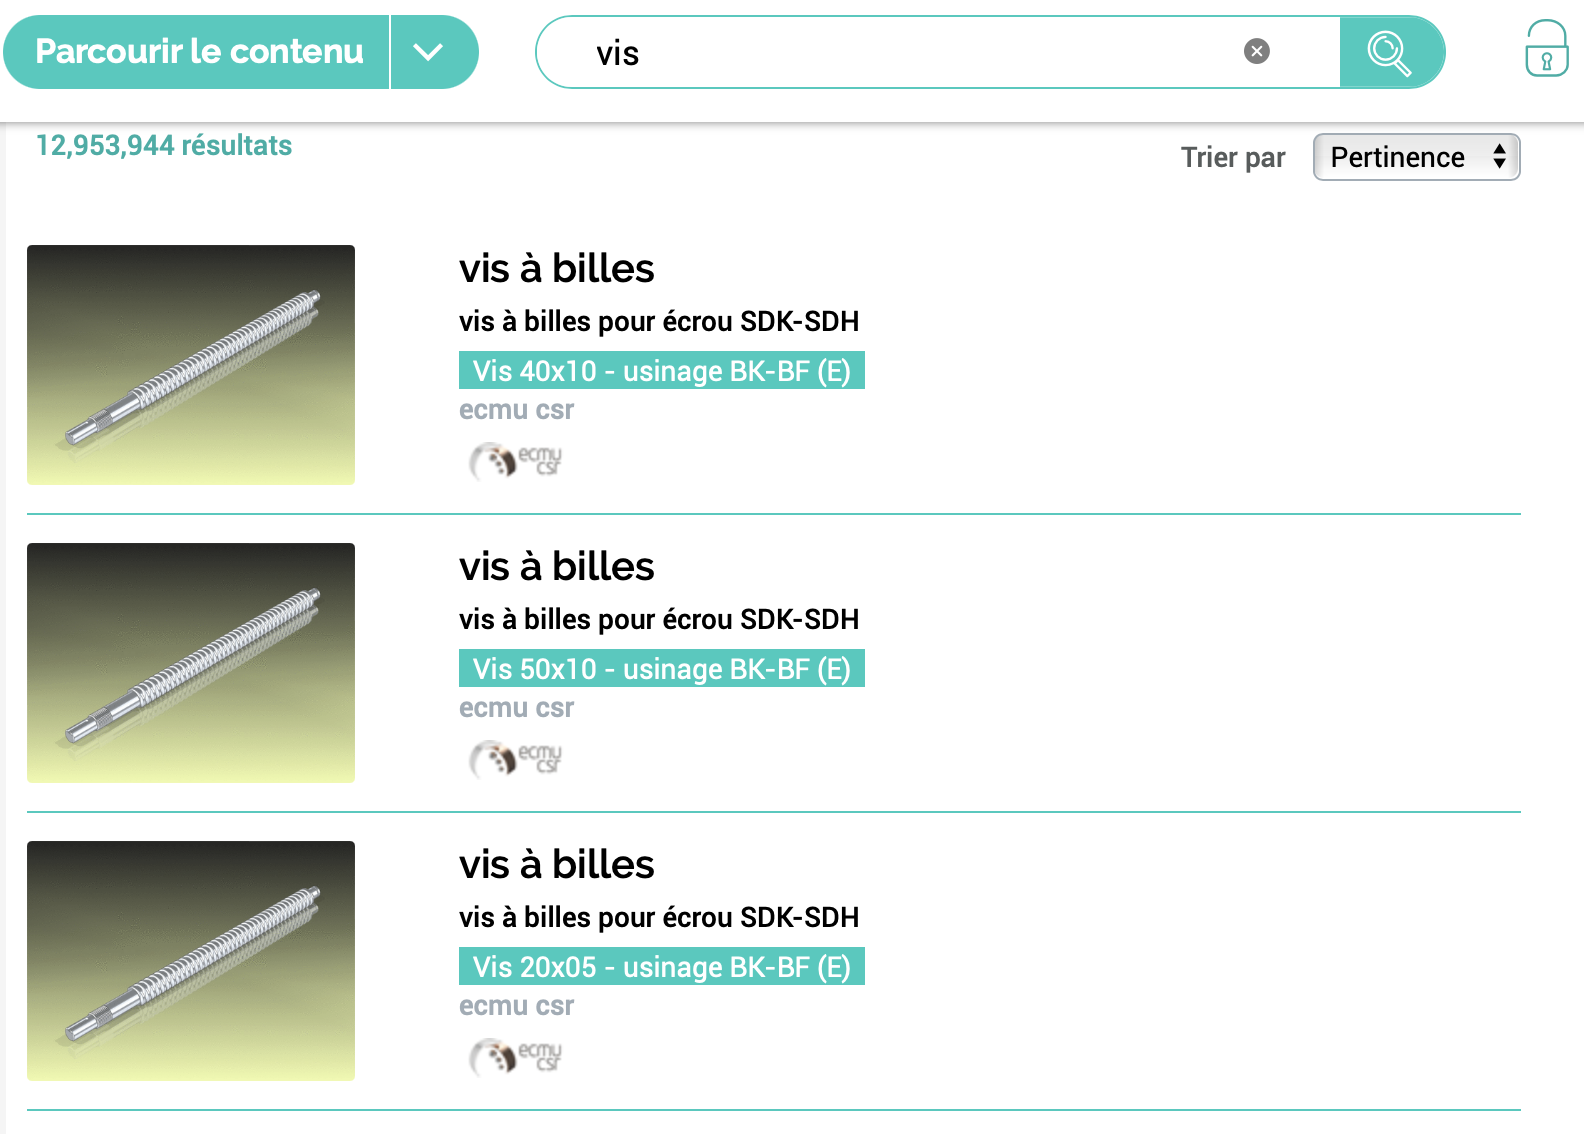
\includegraphics[width=.96\linewidth]{../../resources/se_test_vis.png}
		\caption{SE queried with ``vis''}
		\label{fig:test_es_vis}
	\end{subfigure}
	\caption{Example queries on TraceParts SE}
	\label{fig:tp_se_test}
\end{figure}

\paragraph{Research questions.}
Although ElasticSearch is well-known for its capabilities for fast textual searchess across the 
database entities, we believe that it is not an efficient use of the database to throw a bunch of 
words at it, which can be typed in different languages or formats according to different standards, 
and expect it to fetch satisfactory results. Such a search engine would fail to provide useful and 
proper web resources in so many easily imaginable cases shown below:

\begin{enumerate}
	\item What if the database contained the word ``screw'' but not ``vis''\footnote{``La vis'' means 
		a screw in French.}?
	\item What if the database contained screws but with no proper understanding of the dimensionality 
		of screws?
	\item What if the user query was like ``screwdriver used for small size screws'' and the database 
		had no understanding of whether the user was looking for wrenches, screws, or everything which 
		can be described as small-sized?
\end{enumerate}

The issues mentioned above are the by-product of performing only raw text-based searches across the 
database entities. It is not hard to imagine that some of the entities may contain the same words 
such as ``small'', ``medium'', ``large'', ``dimension'', ``standard'', ``colored'' and so on. Main 
research questions include ``how to make search engines understand necessary distinctions between 
products, products described in their descriptions, their attributes, languages that they are 
expressed in?'', ``what data structure(s) should be used to store data?'', ``how to develop 
algorithms/software to deal with these problems?''.

\paragraph{Research methodology.}
Currently, the search process is blindfolded, meaning that it has no idea what to look for in terms of 
concepts that matter to the user. To avoid such inefficiencies in the run-time performance and ranking 
of the search engine result pages, we can guide the search process by using ontologies and/or 
knowledge graphs \cite{reinanda2020knowledge,dietz2018utilizing,chen2020review}. Knowledge acquisition 
plays a crucial role in the process of developing 
ontologies and/or knowledge graphs. Several approaches to address some of the issues related to 
knowledge acquisition bottlenecks as well as information retrieval systems and search engine 
optimization strategies are demonstrated in chapter \ref{chap:literature}. In this thesis work, 
several knowledge acquisition strategies 
are described for introductory purposes for the following sections. My main contributions in this 
project include the development of a software architecture, implementation of different processing 
paradigms, and building a knowledge acquisition pipeline all of which are introduced and discussed 
thoroughly in chapter \ref{chap:development}. To acquire knowledge from the relational database of 
TraceParts, a relatively simple ontology has been developed and used to build the ultimate knowledge 
graph. The ontology and knowledge graph building process have been described in a more detailed 
fashion later on in the same chapter. In chapter \ref{chap:results_discussions}, implemented library 
and the final software as well as several tests are discussed. Finally, I share my conclusions on 
this project and the internship experiences in chapter \ref{chap:conclusions}.

\paragraph{Practical significance of the thesis.}
The goal of this project work has been dedicated to develop a PoC system with which we could test 
different hyphothesis and compare benchmark results relatively quickly and easily. Such a system would 
play the foundational role in the ultimate search engine version and be sufficient for further 
improvements step-by-step, iteratively.
